\documentclass[12pt,handout]{beamer}
% \documentclass[10pt]{beamer}

% \usetheme{Pittsburgh}
% \usetheme{metropolis}%great
% \usetheme{hsrm}%BEST for Presentation
% \usetheme{Hannover}
% \usetheme{AnnArbor}%good
% \usetheme{Bergen}
% \usetheme{Berkeley}%BEST for Email
% \usetheme{Frankfurt}
\usetheme{Warsaw}% good for risk
% \usetheme{sthlm}

% \usecolortheme{owl} % dark theme
% \usecolortheme[snowy]{owl} % black on white
\usecolortheme[cautious]{owl}% dark wo redef colors

\usepackage{appendixnumberbeamer}
\usepackage[T1]{fontenc}
\usepackage[utf8]{inputenc}
% \usepackage{lmodern}
% \usepackage{tikz} 

% \usepackage{booktabs}
\usepackage[scale=2]{ccicons}

% \usepackage{pgfplots}
% \usepgfplotslibrary{dateplot}

\usepackage{xspace}
\usepackage{tabularx}

\newcommand{\themename}{\textbf{\textsc{metropolis}}\xspace}
\renewcommand\tabularxcolumn[1]{m{#1}}% for vertical centering text in X column

\title{ Hoot Risks and Precautions}
\subtitle{Traversing the various risk curves}
\date{\today}
\author{Hoot AR ads team}
\institute{Hoot Live inc., a Delaware C-corp}
% \titlegraphic{\hfill
\includegraphics[height=1.5cm]{logo.pdf}}

\begin{document}
\maketitle

% \begin{frame}{Table of contents}
% \setbeamertemplate{section in toc}[sections numbered]
% \tableofcontents[hideallsubsections]
% \end{frame}

% \section{Primer}

\begin{frame}[fragile]{Risks and precautions}
	% \begin{itemize}%needs pause
 % \setbeamercovered{transparent}%show dimmed
 % \begin{itemize}[<+->]%uncover piecewise
 \begin{itemize}[<+-| alert@+>]%uncover w highlight 
	 
\item[ ]{Technology Risk }
\begin{itemize}[<+-| alert@+>]
\item one to many at scale completely mitigated, end-to-end solid scalable infrastructure
\item webrtc, p2p, many-to-many, 2 way calling, voice video conferencing
\end{itemize}
\item[ ]{Product Risk}
\begin{itemize}[<+-| alert@+>]
\item provide easy ways to integrate into iOS app in Xcode via Cocoapods
\item provide unity plugins
\item web API and sdks for web-integrations
\item Follow best practices of branchmetrics, amplitude, mixpanel, heroku, open-whisper/signal
\end{itemize}


\end{itemize}

\end{frame}

\begin{frame}[fragile]{Risks mitigation}
 \begin{itemize}[<+-| alert@+>]
\item[ ]Market Risk
\begin{itemize}[<+-| alert@+>]
% \item launch risk
\item Hiring key members to build, drive market adoption
\item Positive response from customers with deep pockets (Linkedin, Disney, Line) 
\end{itemize}

\item[ ]Growth Risk
\begin{itemize}[<+-| alert@+>]
\item targeted hackathons, sponsoring coding schools and code academies
\end{itemize}

\item[ ]Content Risk
\begin{itemize}[<+-| alert@+>]
\item risk of not getting quality content
\item Recruit paid streamers using talent media team who can generate guaranteed viewership and sustained engagement
\item Partner with content/media companies - NFL, Yahoo, MTV, Refinery29, Comedy Central, BuzzFeed, CNN, Cosmopolitan, Vox, People \ldots
\end{itemize}

\iffalse
\item[ ]Team People Risk
\begin{itemize}[<+-| alert@+>]
\item Frank Stanbach → ex roku, apple. expert in Android dev, live-streaming, media
\item Guillaume Pastorino → rtmp, h264, h265 encoder, low-level programming in c, java
\item Hoot Live, inc., can pro-actively build a hiring hit list from Netflix, Twitch, Youtube, Facebook, Yahoo, Twitter, Cisco, Webex, Zoom, Onlive and Google
\end{itemize}
 \fi

\end{itemize}
\end{frame}
\begin{frame}[standout]
 Risks and precautions

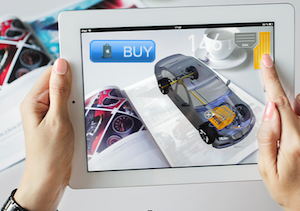
\includegraphics[scale=.2]{static/arad/arad5}

 Traversing risk curve is more important than traversing expense projections. As risks are mitigated burn can be increased 


 
\end{frame}

\end{document}
